\documentclass[french]{article}
\usepackage[utf8]{inputenc}
\usepackage{babel}
\usepackage{graphicx}
\usepackage{caption}
\DeclareCaptionLabelSeparator{as-Babel-french}{\space\textendash\space}
\captionsetup{labelsep=as-Babel-french}
\captionsetup[table]{position=top}
\newcommand\multi[2]{\multicolumn{1}{#1}{#1}}
\begin{document}
	Le tableau~\ref{t:prix_materiaux} et la figure~\ref{f:echantillons} illustrent l'utilisation 
	d'objets flottants qui sont positionnés immédiatement après le texte. Comme il se doit dans 
	un texte en français, la légende du tableau le précède, alors que celle de la figure la suit.
	\begin{table}[htp]	 \caption{Liste de prix des matériaux de référence au 1 février 2006, minérales (LMSM).}
		\centering
		\label{t:prix_materiaux}
		\begin{tabular}{|l|c|r|} \hline\hline
			\multi{|c|}{\emph{description}} & \emph{unité} & \multi{c|}{\emph{prix}}
			\\ \hline
			Minerai d'uranium          & 100 g     &   95,00  \$ \\
			Minerai d'or               & 200 g     &  180,00  \$ \\
			Alliages de zinc-aluminium & 7 disques & 1500,00 \$ \\
			\hline\hline
		\end{tabular}
	\end{table}
	\begin{figure} % top par défaut
		\centering
		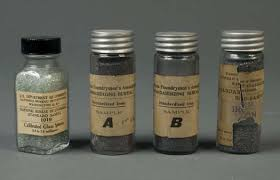
\includegraphics[width=0.5\textwidth]{mat}
		\caption{Les matériaux de référence se présentent sous forme d'échantillons en
			poudre de minerais, de roches, de sédiments, de sols, de concentrés et de
			produits de traitement, dont la composition chimique a été établie avec
			précision.} 		\label{f:echantillons}
	\end{figure}
\end{document}